%!TEX root = ../Thesis.tex
\chapter{Relevant Background}
\label{chap:reletiveBackground}

\section{Depth Perception}
Depth perception is the ability of the Human Visual System \index{HVS} to visualize the three dimensional world as well as measuring the distance of an object based on two dimensional images obtained from the eyes. Depth perception is imperative for performing basic everyday tasks such as avoiding obstacles without bumping into them or interacting with the world with relative ease. In animals (specially predators), it is critical to estimate the distance of a prey for an efficient attack. Depth sensation is the term used for animals as it is not known whether they sense the depth in the same way as humans do or not\cite{ wiki:depth_perception}.

% Figure for cues
\begin{figure}
\begin{tikzpicture}[grow'=right,level distance=1.75in,sibling distance=.15in]
\tikzset{edge from parent/.style = {thick, draw, edge from parent fork right},
         every tree node/.style  = {draw,minimum width=1in,text width=1.3in,align=center}}
\Tree
    [. {Depth Information}
	        [.{Monocular Cues}
	                [.{Motion Parallax } ]
	            	[.{Depth from Motion } ]
	            	[.{Kinetic Depth Effect } ]
	            	[.{Perspective } ]
	            	[.{Relative Size} ]
	            	[.{Familiar Size} ]
	            	[.{Absolute Size} ]
	            	[.{Ariel Perspective} ]
	            	[.{Accommodation} ]
	            	[.{Occlusion} ]
	            	[.{Curvilinear Perspective} ]
	            	[.{Texture Gradient} ]
	            	[.{Shading} ]
	            	[.{Defocus Blur} ]
	            	[.{Elevation} ]
	        ]
	        [.{Binocular Cues}
	                [.{Stereopsis } ]
		            [.{Convergence } ]
		            [.{Shadow Stereopsis} ]
	        ]
    ]
\end{tikzpicture}
\caption{HVS Depth Cues\label{fig:CueTree}}
\end{figure}

Human visual system \index{HVS} uses several monocular and binocular cues to determine the depth of objects in the view. These cues can be categorized into two categories i.e. cues extracted from a single image (Monocular Cues) and cues extracted from two images (Binocular cues)\cite{depthcues1}\cite{ wiki:depth_perception}. Figure \ref{fig:CueTree} gives an outlook of the depth cues used by the HVS. These cues are then dynamically weighted according to their robustness by the HVS in order to estimate a depth value for each object in the view \cite{CueFusion}(Write details of those cues in Appendix).


\section{Binocular Vision and Stereopsis}
% Limits of stereopsis and that other paper of bank.\cite{banks1}
% cormack paper.
% when fusion and happens and when not and why?
Generally speaking, all the animals with two eyes have binocular vision and they can integrate the information from two eyes based on the binocular overlap. But the term Binocular vision is usually used for the animals that have a large area of binocular overlap (Human and most other predators) and use it to get the depth information of the world around them. In addition to calculating depth, binocular vision also has advantages in performing other tasks such as detection, discrimination, detecting camouflaged objects or eye-hand coordination. Even the resolution observed world is increased with binocular vision\cite{howard1995binocular}. Among all the depth cues discussed in the section above, Stereopsis is the most influential of them all. Since the human eyes are located at different lateral positions on the head, the images formed on the retinas of these two eyes are slightly different. The difference is mainly the horizontal positions of the objects\cite{ wiki:stereopsis}. The process of obtaining a fused (Binocular fusion) image (Cyclopean image) and obtaining a depth map based on the horizontal disparities of the objects in these two images is known as stereopsis.

When the eyes verge in order to focus on some object (or point) in space, that object is projected at identical corresponding points in the retinas. It means that the difference between their horizontal positions is zero. This process is called fixation of the eyes and the distance of the object (point) at which the eyes are fixated is called the fixation distance. The locus of all the points in space that is projected on identical retinal points is called the horoptor\cite{ wiki:horoptor}. Theoretically, via geometrical principles, the horoptor is a circular segment in the plane of fixation point. However, Wheatstone in 1938 observed that the actual/emperical horopter is much larger than that. Figure \ref{fig:horoptor} shows both the theoretical and empirical horoptor. Any object that is farther away from the horoptor has uncrossed disparity in the retinas i.e. the eyes need to be diverged (uncrossed) in order to fixate on that object. Similarly, any object that is closer than the horoptor has crossed disparity in the retinas i.e. the eyes need to be converged (further crossed) in order to fixate at it \textcolor{red}{cite and make the diagram for crossed uncrossed disparities}. Figure ?? shows a graphical representation of crossed and uncrossed disparities \textcolor{red}{add the dolphin images from wikipedia article.}.

\begin{figure}
\centering
    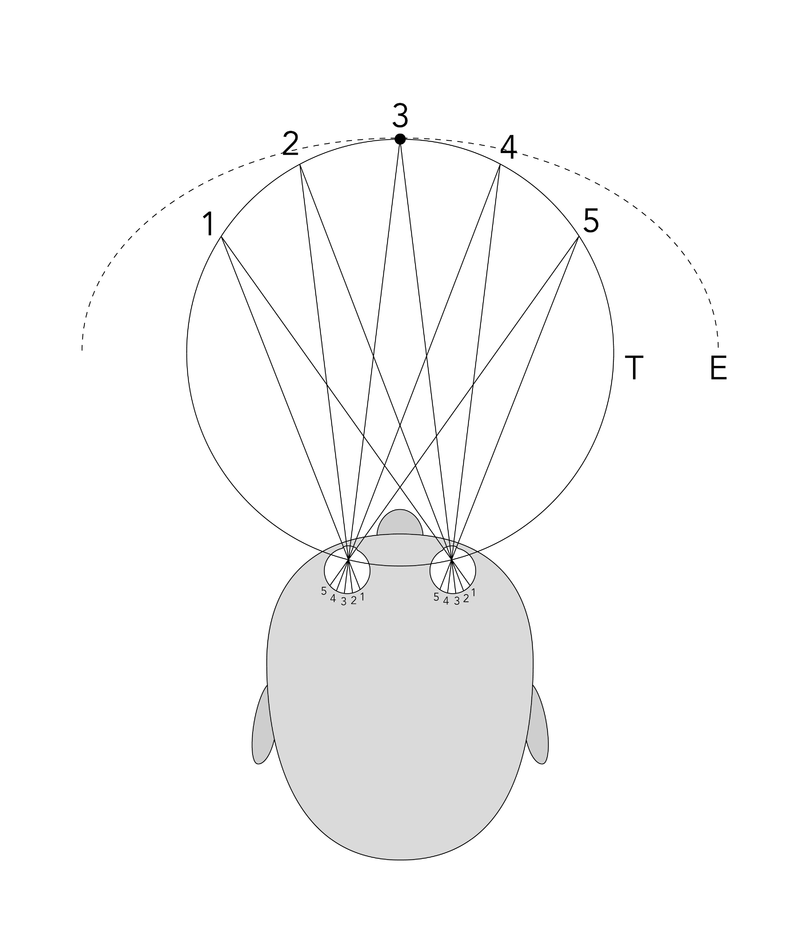
\includegraphics[width=0.5\textwidth]{./Template_Figures/horopter}
    \caption{Representation of theoretical (T) and empirical (E) horoptor\label{fig:horoptor}}
\end{figure}

Stereopsis is believed to be processed in the binocular neurons of the visual cortex of mammals. The binocular neurons have receptive fields in different horizontal positions in each eye. These cells are active only when the object of interest is in certain range of disparity in one eye relative to the other i.e. there is a maximum disparity limit. \textcolor{red}{add the dolphin images from wikipedia article.}. As the objects in the images formed at the retinas of both eyes are slightly shifted horizontally, presenting two different images with shifted object two both eyes can fool the HVS into perceiving depth. This process is called stereoscopy. The first stereoscope was invented by Sir Charles Wheatstone in 1838\cite{ wiki:wheatstone}. It used two mirror both tilted at 45 degrees to the eyes that reflected two different images from the sides. Currently all the stereoscopic screen present a different perspective image two both eyes with different technologies that will be discussed in later sections.

\section{Limits of Stereopsis}
% Limits of stereopsis and that other paper of bank.\cite{banks1}
% cormack paper.
% when fusion and happens and when not and why?









\section{Crosstalk}
% Definitions and Factors contributing to Crosstalk
% Effects on viewers
% 70\% thing etc.
As discussed in the previous section, stereoscopy includes the process of displaying different perspective images to each eye in order to mimic the effect of depth in a scene. However, it is critical that the perspective of these two images should be segregated completely from each other. Currently, all the commercially available 3D displays (with exception of head mounted displays or Wheatstone setups) fail to isolate the two images completely. That means that a percentage of the image of one eye leaks to the other eye as well. This unintended leakage is called the crosstalk in stereoscopic screens\cite{woods2012crosstalk}. Figure \ref{fig:ct1} Shows one such example where the screen has a simulated crosstalk of 14\%. This means that 14\% image intensity of the right eye image is leaked into the left eye image and vice versa.

\begin{figure}[htbp]
    \centering
    \begin{subfigure}[b]{0.3\textwidth}
        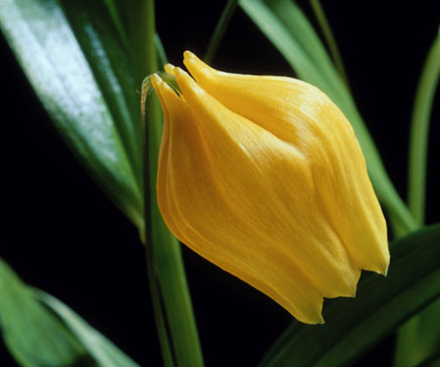
\includegraphics[width=\textwidth]{./Template_Figures/orig}
        \caption{Original Image}\label{originalPicture}
    \end{subfigure}
    \begin{subfigure}[b]{0.3\textwidth}
        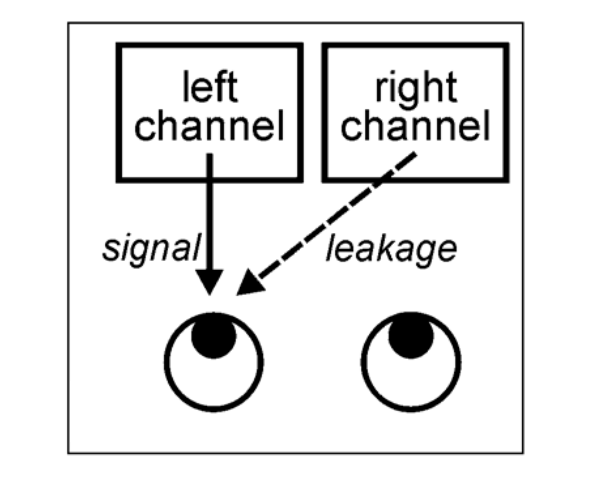
\includegraphics[width=\textwidth]{./Template_Figures/leakage}
        \caption{Original Image}\label{ill_leackage}
    \end{subfigure}
    \begin{subfigure}[b]{0.3\textwidth}
        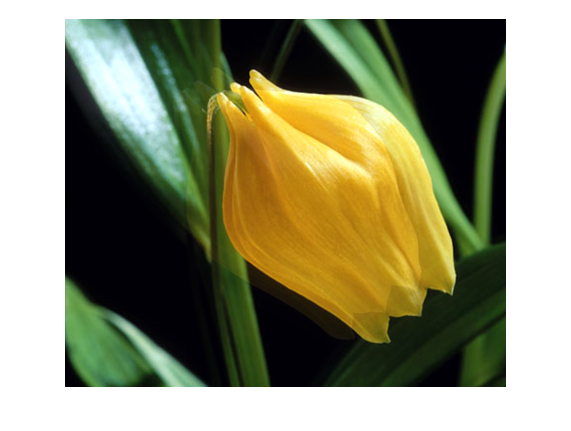
\includegraphics[width=\textwidth]{./Template_Figures/crosstalk}
        \caption{Original Image}\label{imWCT}
    \end{subfigure}
    \caption{A simulation of 14\% crosstalk. An Image intended for the left eye containing 14\% of image intended for right eye. containing \label{fig:ct1}}
\end{figure}

System crosstalk is the term used to define the amount of light leakage that occurs between two views. In simplest form, it can be mathematically defined as:

\begin{equation}
Crosstalk(\%) = \frac{leakage}{signal} *100
\label{eq:simple_crosstalk}
\end{equation}

Here, \say{signal} is the luminance of the original image intended for an eye and \say{leakage} is the luminance of the light that leaks from the unintended image. Usually, on a stereoscopic scree, the amount of crosstalk is measured by observing the luminance of the left channel while a black (minimum luminance) image is displayed in the left channel and a white (maximum luminance) image is displayed on the right channel and vice versa. This definition is accurate for the screens that can manage to display a true black i.e. zero luminance. Almost all of the LCDs can not produce zero luminance as their minimum luminance hence resulting in a non-zero black level at its minimum. Another mathematical representation of crosstalk take into effect this non-zero black level and is defined as:

\begin{equation}
Crosstalk(\%) = \frac{leakage - black level}{signal - black level} *100
\label{eq:crosstalk_gray}
\end{equation}

Throughout the rest of the paper, we will be using crosstalk as mentioned in eq \ref{eq:crosstalk_gray}.

\section{Stereoscopic/Automultiscopic Screens and its cross-talk}
\subsection{CRT Screens}
\subsection{LCD Screens}
\subsection{Anaglyph Stereo}
\subsection{Active/Time Sequential Stereo}
\subsection{Passive/ Space Multiplexed Stereo}
\subsection{Automultiscopic Screens}

\section{Crosstalk Quality Metrics}

\section{Lightfields}